\section{Renewable Energy 2 Time Series} \label{sec:renewable2}

This subsection presents a contextualization, contributions, datasets, and methodology adopted for application 3.

\subsection{Contextualization and Contributions}

Over the past few decades, wind energy in many nations worldwide has increased its role in the energy matrix. Between 2020 and 2024, the Global Wind Energy Council anticipates that more than 355 $GW$ of new capacity will be installed, including about 71 $GW$ of new plants every year up to 2024 \cite{globalwindenergycouncilgwec2020Market}. Wind power, including in Brazil, has a considerable part of the national energy grid. The electric energy system mainly comprises hydroelectric energy (57.8\% of energy output), one of the primary renewable energy sources. In line with the \citeonline{brazilianwindenergyassociationabeeolica2021Energia} study of 2021, ``Infowind'', as of February 2021, Brazil is now 7th in the world with 18 $GW$ of installed wind energy capacity from more than 8,300 wind-energy turbines, spread throughout 695 wind farm areas on the coast of Brazil. Wind energy generated 55,9 $TWh$ in 2019, an increase of 15.5\% over the previous year. This generation feeds 88.5 million people and accounts for 17\% of the total energy utilized in the interconnected national network.

Notwithstanding the wind energy expansion, the central issue is the electricity grid's reliability since wind energy generation can once swing between 20 and 100 percent of the wind farm's capability owing to intermittent wind properties \cite{vatanpour2018Impact}. In different terms, wind energy is identified as an intermittent source, making its supply unpredictable due to the high level of insecurity and the nonlinear behavior of the wind speed \cite{dasilva2021Novel}. The \ac{ONS} primary key is establishing reliable wind speed forecasts to plan daily electrical energy dispatch. That avoids or limits system stability and frequency regulation impacts and lowers wind energy curtailment surplus \cite{moreno2020Multistep}.

Therefore, an accurate wind speed forecast is crucial for asset management and the electrical system operator. Wind speed forecasting across various horizons is critical for turbine regulation, electricity market clearing, energy allocation, electric power management, and equipment maintenance schedules. Wind speed prediction models may also be categorized into four groups, very short, short, medium, and long-term, by their predicted time horizon \cite{liu2019Data}. A shorter prediction time frame may produce more comprehensive and accurate findings, but there is less time for deploying wind power generation. On the other hand, a lengthier forecasting time horizon gives long-term knowledge on future wind energy, but the accuracy is typically decreased \cite{moreno2019Very}.

Forecasting short-term wind speed as precisely as possible is essential to the energy market and \ac{ONS} due to wind characteristics and the present Brazilian electrical system condition. Therefore, this study aims to offer a hybrid forecasting system that combines \ac{SSA} and \ac{VMD} with machine learning methods and \ac{STACK}. The model will train the elements obtained in the decomposition, striving to forecast the short-term wind speed in a multi-step manner (10, 30, and 60 minutes ahead horizon). In consideration of those as mentioned above, the following \ac{RQ}s are defined:

\begin{enumerate}[wide=0pt, leftmargin=3em]
    \item[\textbf{RQ 1.3}] Can signal decomposition approaches enhance the performance of forecasting wind speed time series?

    \item[\textbf{RQ 3.2}] What is the improvement achieved by employing \ac{STACK} approach coupled with signal decomposition approaches over non-decomposed models when forecasting wind speed time series?

    \item[\textbf{RQ 5}] Can the multi-stage signal decomposition strategy outperform the single-stage signal decomposition approach?

    \item[\textbf{RQ 6}] Can the employment of \ac{STACK} method improve the forecasting performance of the multi-stage signal decomposition strategy?
\end{enumerate}

To address the \ac{RQ}s of this application, the contributions can be summarized as follows:

\begin{enumerate}[label=\alph*)]

    \item The use of multi-stage signal decomposition for short-term wind speed forecasting. Combining two decomposition techniques (\ac{SSA} and \ac{VMD}) to compose a two-stage signal decomposition technique, the \ac{VMD} performed the first stage, and \ac{SSA} performed the second stage. This process is also evaluated accordingly.
    
    \item The use of the stacked generalization ensemble learning framework coupled with multi-stage signal decomposition for short-term wind speed forecasting. The stacking-ensemble learning scheme can enhance the performance of the multi-stage signal decomposition framework by its divide-and-conquer characteristic, making the model more robust.
    
    \item Using different machine learning forecasting models combined with the multi-stage signal decomposition and stacking-ensemble learning approaches. The reason for choosing different models to compose the \ac{STACK} model is due to the diversity of the models' characteristics, in which the \ac{STACK} approach can extract the best from each model.
    
\end{enumerate}

\subsection{Dataset Description}

The dataset utilized as input in the proposed framework consists of three months of wind speed measurements. The measurements are made every 10 min at a height 95 meters from ground level, corresponding to a wind generator with a blade diameter of 100 meters. The measurement apparatus is installed to monitor the wind resource for a wind farm, with approximately 150 $MW$ capacity, located in the State of Rio Grande do Norte, in the Northeastern region of Brazil, more specifically at Parazinho city. The measurements are made from March until May 2020. The time series is created out of 4,464 samples for March and May 2020 and 4,320 samples for April 2020, with a sampling period of 10 min, as presented in Figure~\ref{fig:datasets}. Using data from different months is essential because further data permit models to learn the maximum number of data features. Also, it has its climatic characteristics each month and thus makes it possible to assess the pattern in various climate situations \cite{dasilva2021Novel}. Furthermore, once the data came from a private company the datasets are limited to these periods.

% Figure - datasets
\begin{figure}[htb!]
    \centering
    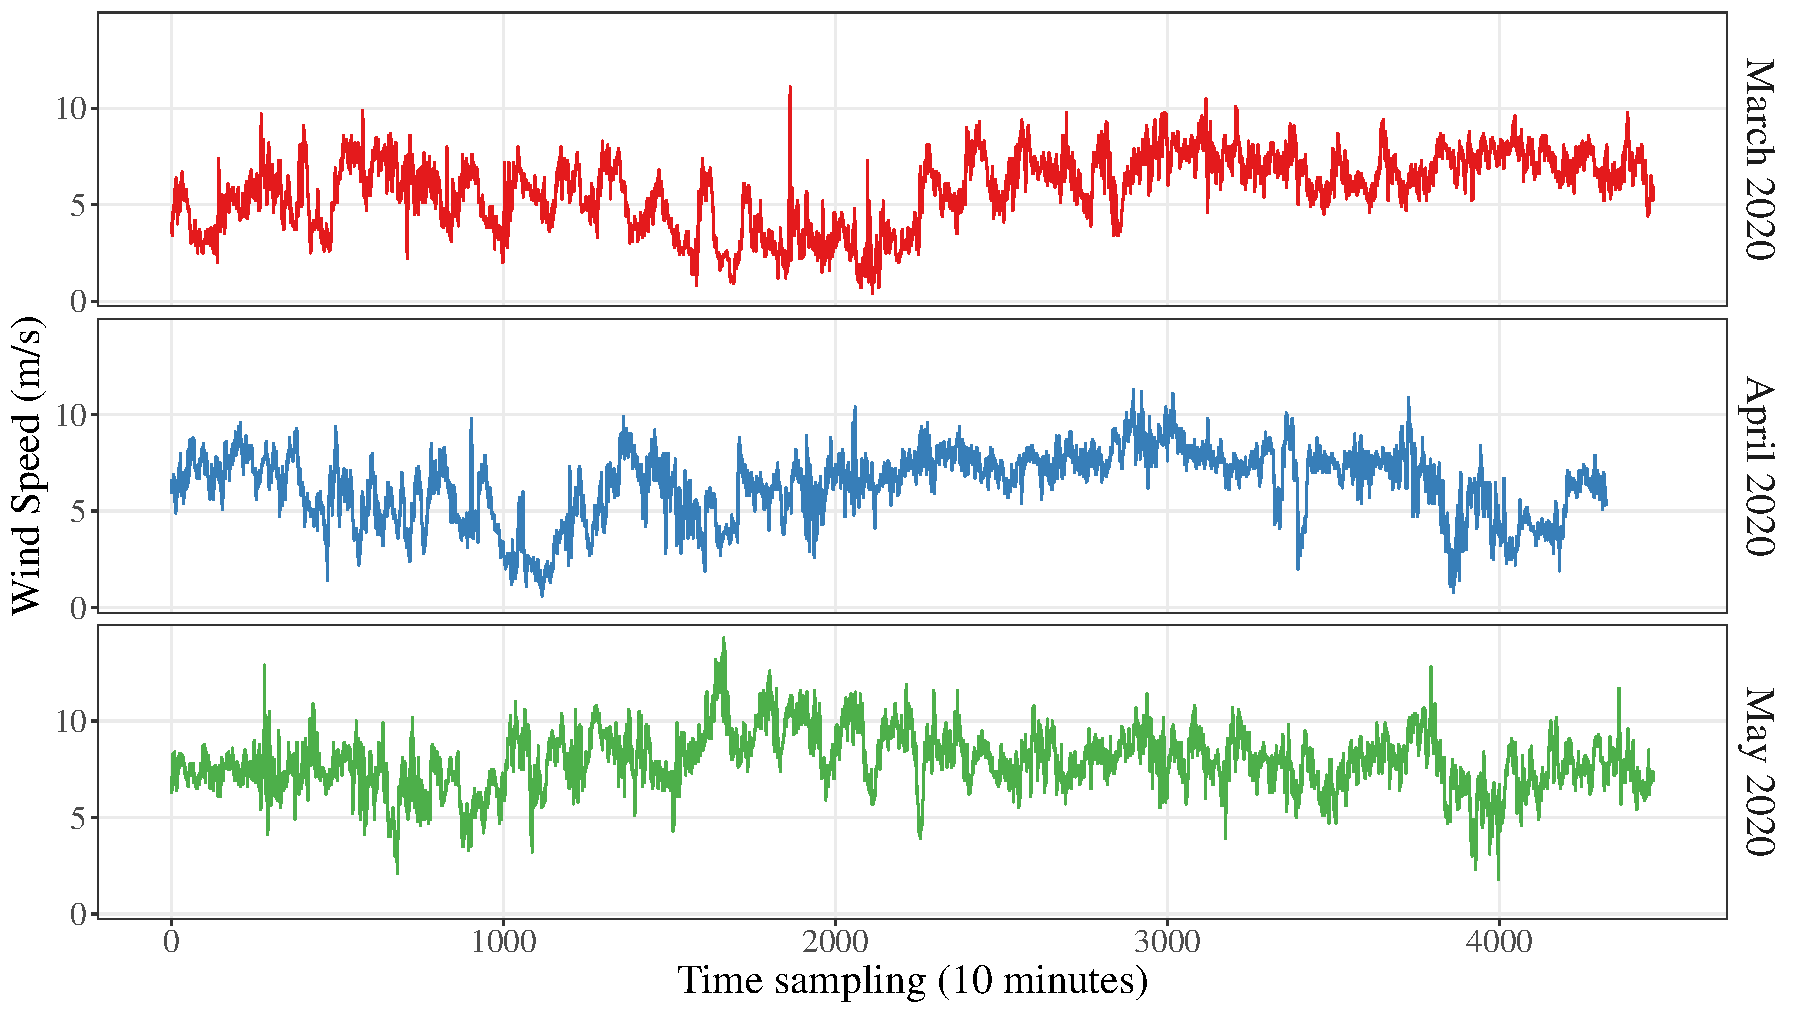
\includegraphics[width=\linewidth]{Media/cs3_datasets_plot.pdf}
    \caption{Datasets for March, April, and May 2020, respectively}
    \label{fig:datasets}
    \source{\citeonline{dasilva2022Multistep}}
\end{figure}

Moreover, the datasets were sequentially divided into training and test sets for three and one weeks. Then, the test set, corresponding to the out-of-sample data, and composed of the last seven days of the month, has about 1,008 observations each month. Those proportions were enough so that models could learn the patterns and behavior of the data, with a sufficient number of observations to give a fair number of points to evaluate the learning procedure. Also, other proportions used in the literature were analysed such as 80 and 20\%, 75 and 25\%, and 70 and 30\%, however the proportion of three weeks for training set and one week for test was chosen due to interpretability and usability of the model by the company that provided the data.

\subsection{Proposed Forecasting Framework}

The proposed model is made out of two decomposition stages. First, the decomposition using \ac{VMD}, and, subsequently, the decomposition using \ac{SSA}. \ac{VMD} extracts the trend components from each original dataset output. The remaining signal is decomposed into four other parts using \ac{SSA}, so each time series is decomposed into five components by \ac{VMD} and \ac{SSA}.

The \ac{RIDGE}, \ac{KNN}, \ac{SVR} with linear kernel, and \ac{PLS} are evaluated as the layer-0 base learners in the training process. In layer-1, the \ac{CUBIST} model is trained. The predictions of each component of layer-0 are added (for every individual model) to form each model's forecast. The predictions of the base learners are used as input for the layer-1 meta-learner. The predictions of the meta-learner form this study's proposed model named \ac{VMD}--\ac{SSA}--\ac{STACK}. The models' performances are evaluated by using \ac{IP}, \ac{MAE}, \ac{MAPE}, \ac{RMSE}, \ac{RRMSE}, and \ac{SSE} performance metrics. Furthermore, the \ac{DM} hypothesis test is employed to evaluate the statistical significance of the difference in errors of the models. The framework for the proposed model is illustrated in Figure~\ref{fig:framework} and explained in further detail in the following steps.

% Figure - Framework
\begin{figure}[htb!]
    \centering
    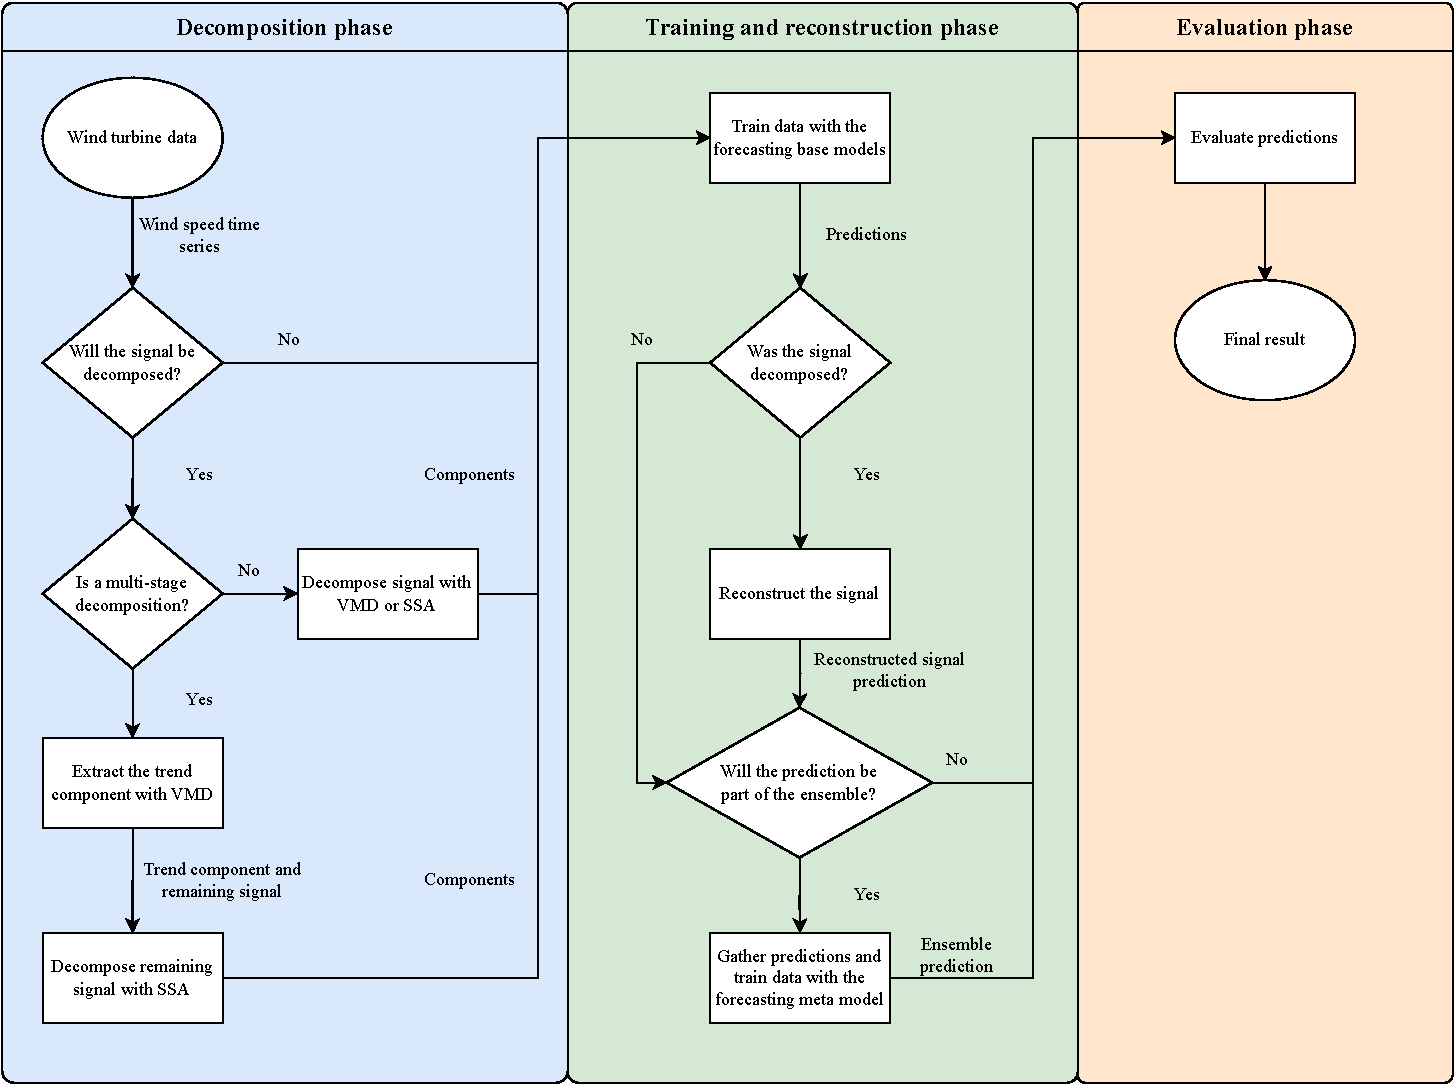
\includegraphics[width=\textwidth]{Media/cs3_framework.pdf}
    \caption{Proposed forecasting framework for Application 3}
    \label{fig:framework}
    \source{\citeonline{dasilva2022Multistep}}
\end{figure}

\begin{enumerate}[start=1,label={\textbf{Step \arabic*:}},wide = 0pt, leftmargin = 3em]
\item First, the \ac{VMD} was performed to extract the trend component ($c_1$) from the original time series. The difference between the original time series and $c_1$ was calculated, resulting in a high-frequency signal. \ac{SSA} decomposed this remaining signal into four other components ($c_2$ up to $c_5$). The main idea of the hybrid multi-stage decomposition is to use \ac{VMD} as the first decomposition method due to its characteristic of dealing with high oscillatory signals by suppressing the high-frequency noise from the components generated. Therefore, \ac{VMD} extracts the band-limited trend component from the signal, while the \ac{SSA} decomposes the remaining signal into a trend, seasonal, oscillations, and aperiodic noises. The five components are presented in Figure~\ref{fig:comps}.

% Figure - components
\begin{figure}[htb!]
    \centering
    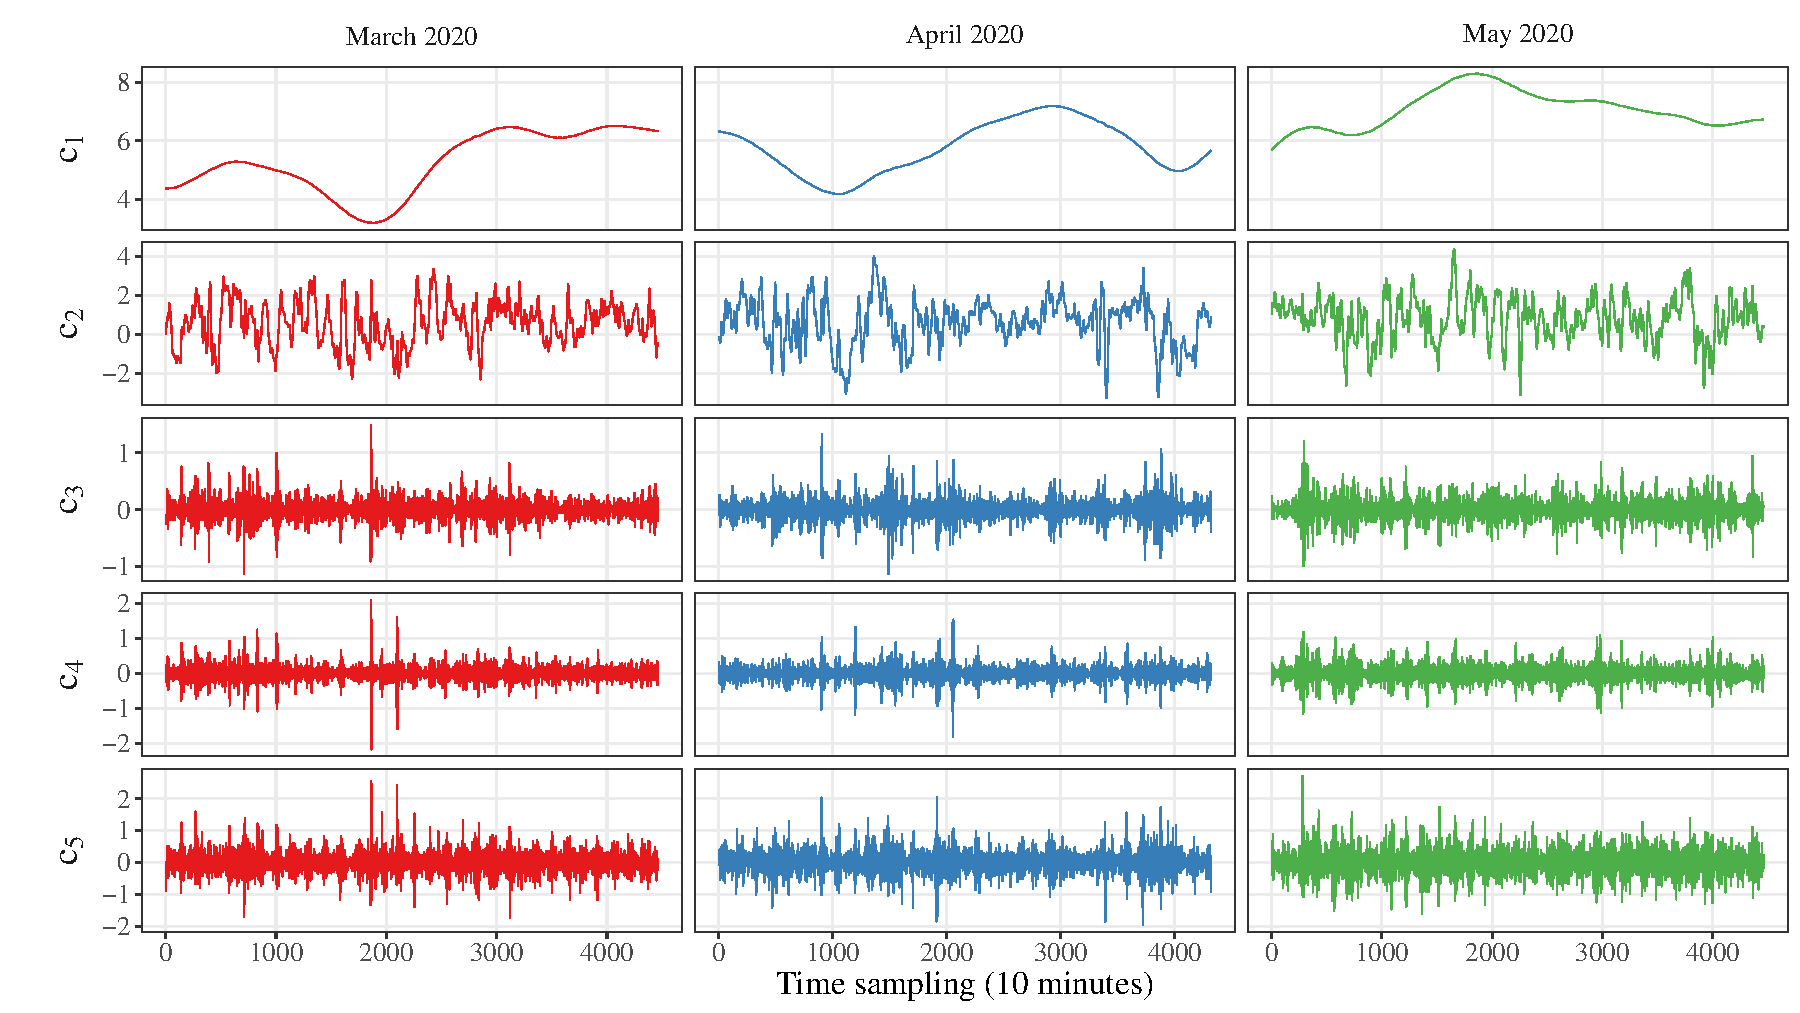
\includegraphics[width=\linewidth]{Media/cs3_imf_plot.pdf}
    \caption{Datasets decomposed into components by VMD and SSA approaches}
    \label{fig:comps}
    \source{\citeonline{dasilva2022Multistep}}
\end{figure}

The value of 5 lags was determined via grid-search and used to transform the data into a format suited to supervised learning models. The data is then split into train and test sets. The test data is made from the last 1,008 measurements, which are the previous seven days of the dataset, while the training is performed with the remaining samples. The train and test sets are in the proportion of 77.5\% and 22.5\%, respectively, sufficient for the models to learn data patterns in the problem in this study. Parameters for \ac{VMD} and \ac{SSA} decomposition are shown in Table \ref{tab:settings} on Appendix~\ref{app:hyper3}. For \ac{SSA}, $C$ is the number of components of the \ac{SSA} procedure, and $n$ is the length of the time series. Regarding \ac{VMD}, $\alpha$ is the balancing parameter of the data fidelity constraint, $\tau$ is the time-step of the dual ascent (usually we can pick 0 for noise-slack), $k$ the number of modes to be recovered from \ac{VMD}, and the iteration number which is triggered if do not converge at tolerance level.

In a scheme in which each component is predicted individually, like the one used in this study and shown in Figure \ref{fig:framework}, the relationship between the number of components and the number of parameters needs to be addressed as more models result in more parameters \cite{moreno2020Multistep}. It is possible to analyze the contribution of every eigenvalue $\lambda_i$ from the singular value decomposition to determine the number of resulting components from the decomposition procedures, which is related to how much each one contributes to the complete time series. This contribution can be estimated by
%
\begin{equation}
    \textit{\%Contribution} = \frac{\lambda_i}{\sum_{i=1}^{l}\lambda_i}.
    \label{eq:eigen}
\end{equation}

% Figure - spectrum
\begin{figure}[htb!]
    \centering
    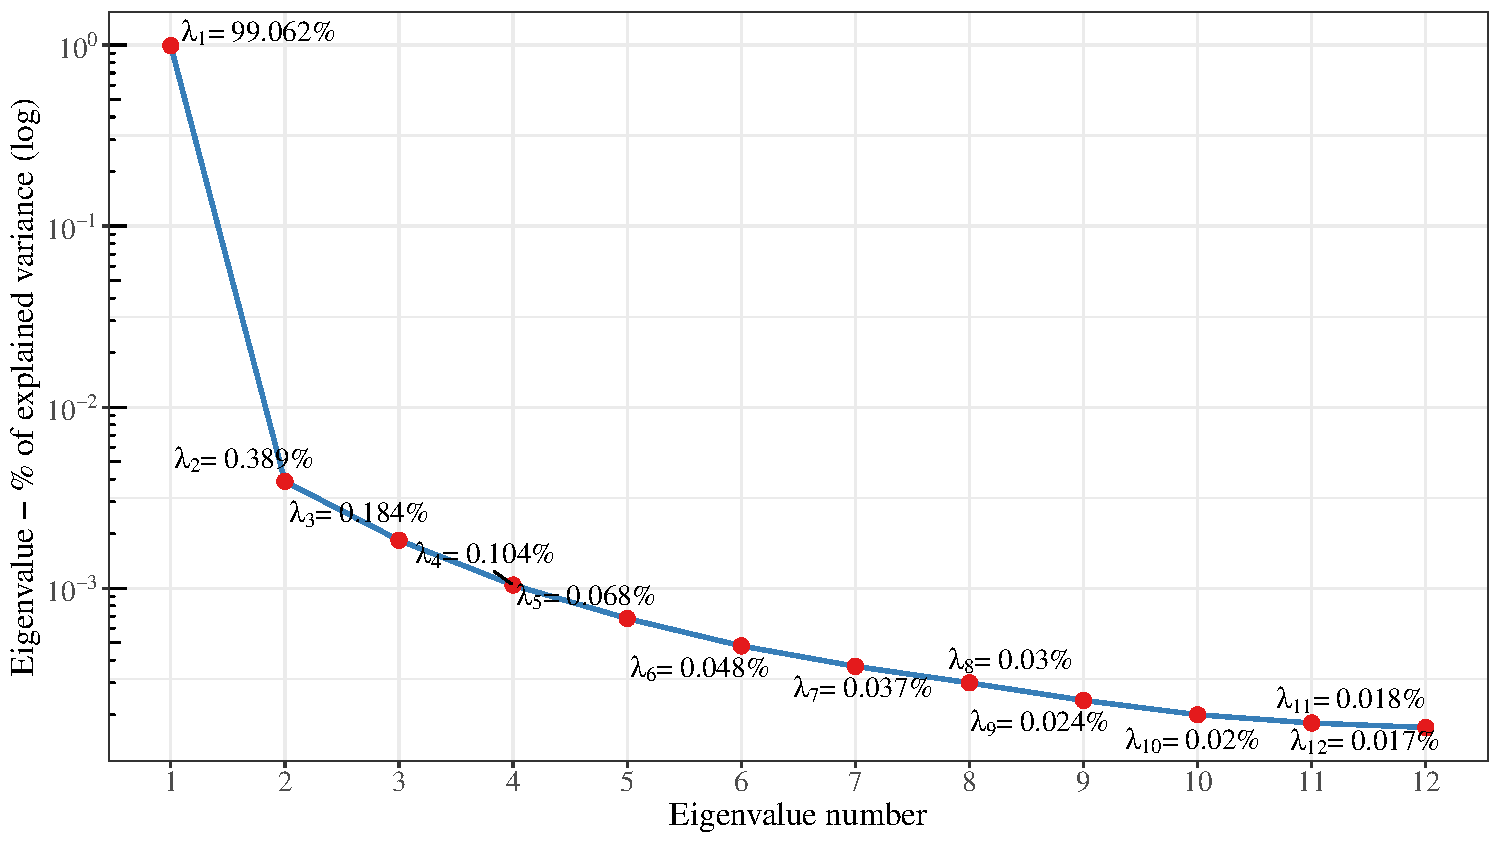
\includegraphics[width=.9\linewidth]{Media/cs3_spectrum.pdf}
    \caption{Explained variance by each eigenvalue number}
    \label{fig:spectrum}
    \source{\citeonline{dasilva2022Multistep}}
\end{figure}

Figure \ref{fig:spectrum} shows the contribution of every eigenvalue for the time series of March 2020. The contribution is considerably small after the second eigenvalue ($\lambda_2$). After the fifth eigenvalue, the sum of contributions is equal to 0.194\%. According to \citeonline{moreno2020Multistep}, this is an important metric to make a better decision considering the trade-off where increasing the number of components it will increase the number of parameters related to forecasting model that needed to be adjusted. Hence, using this analysis helps determine how much adding new parameters to the model by adding new components could help to improve the results further. As shown in Figure \ref{fig:spectrum}, the number of five components was chosen since, according to this analysis, it could explain 99.81\% of the variance of the time series.

\item For every component, the models aforementioned were trained using a 5-fold cross-validation, as in \citeonline{ribeiro2022Efficient} and \citeonline{dasilva2021Novel}, forming the base-models of the \ac{STACK}. Subsequently, the component predictions for every model are summed up by the model, creating forecasts for the single models with decomposition. With this, the four single models with decomposition predictions are generated: \ac{VMD}--\ac{SSA}--\ac{KNN}, \ac{VMD}--\ac{SSA}--\ac{PLS}, \ac{VMD}--\ac{SSA}--\ac{RIDGE}, and \ac{VMD}--\ac{SSA}--\ac{SVR}.

\item The prediction outputs from base-learners (layer-0) are used as input for the \ac{STACK}'s top layer (layer-1) meta-learner training. The meta-learner was built using a \ac{CUBIST} model. These predictions are then the predictions of the proposed model, named \ac{VMD}--\ac{SSA}--\ac{STACK}. Moreover, Table \ref{tab:hyperparameters} on Appendix~\ref{app:hyper3} shows the proposed model's hyperparameters for this study. These are the hyperparameters for every model, dataset, and forecasting horizon. The hyperparameters were defined using a grid-search for the base learners and the meta-learner.

\item A recursive strategy is utilized for multi-step ahead forecasts of this work \cite{dasilva2021Novel}. For this method, the model is fitted to a one-step-ahead forecast. The output of the first step is used as input for the second step. This process is repeated as often as needed to achieve the desired horizon. The forecast value in $t+1$ is always used to obtain the forecast in $t+2$ and subsequently for the next steps, with $t$ as the present time. This scheme is represented in Figure \ref{fig:recursive}, where the blue color represents the known actual values, the green color represents the values from the forecast of previous steps, and the yellow color represents the value being predicted in the given stage. Using this configuration, for a six-steps ahead forecast and five lagged values as input, none of the inputs are actual observed values by the sixth step ($t+6$), and only forecast values of previous steps are considered.

% Figure - recursive framework
\begin{figure}[htb!]
    \centering
    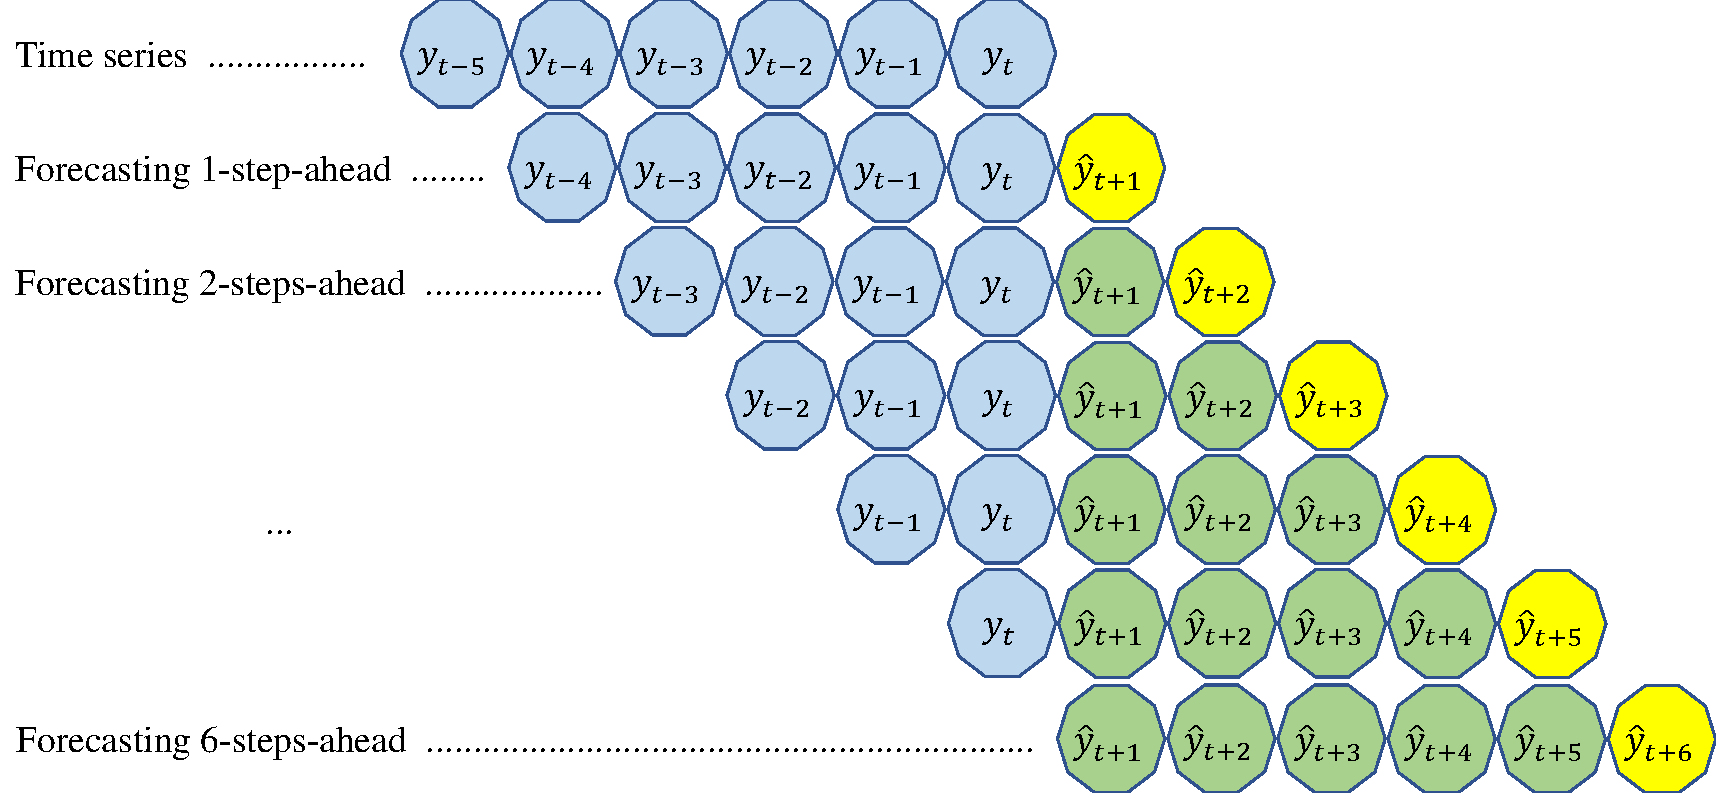
\includegraphics[width=0.85\textwidth]{Media/cs3_recursive-diagram.pdf}
    \caption{Recursive strategy of forecasting exemplified for 6-steps ahead}
    \label{fig:recursive}
    \source{\citeonline{dasilva2022Multistep}}
\end{figure}

In this study, forecasts for the $H$ next step are possible for the proposed model. For the analysis, forecasts for one, three, and six steps are produced. The following equation represents the structure for each horizon,

\begin{equation}
    \hat{y}_{(t+h)} =
    \begin{cases}
    % \left\{\begin{array}{ll}
    \hat{f}\left\{{y}_{(t+h-1)},\,{y}_{(t+h-2)},\,{y}_{(t+h-3)},\,{y}_{(t+h-4)},\,{y}_{(t+h-5)}\right\} & \textnormal{if } h = 1, \\
    \hat{f}\left\{\hat{y}_{(t+h-1)},\,\hat{y}_{(t+h-2)},\,{y}_{(t+h-3)},\,{y}_{(t+h-4)},\,{y}_{(t+h-5)}\right\} & \textnormal{if } h = 3, \\
    \hat{f}\left\{\hat{y}_{(t+h-1)},\,\hat{y}_{(t+h-2)},\,\hat{y}_{(t+h-3)},\,\hat{y}_{(t+h-4)},\,\hat{y}_{(t+h-5)}\right\} & \textnormal{if } h = 6, \\
    % \end{array}
    % \right.
    \end{cases}
\end{equation}
where $\hat{f}$ is a function that maps the wind speed, $\hat{y}_{(t+h)}$ is the forecast of wind speed in time $t$ in horizon $h=$1, 3, and 6, $y_{(t+h-1)}$ up to $y_{(t+h-5)}$ are the previous observed, $\hat{y}_{(t+h-1)}$ up to $\hat{y}_{(t+h-5)}$ are the predicted wind speed.

\item To evaluate the effectiveness of adopted models, the \ac{IP}, \ac{MAE}, \ac{MAPE}, \ac{RMSE}, \ac{RRMSE}, and \ac{SSE} performance criteria are performed. Furthermore, a \ac{DM} test is conducted to evaluate whether or not the forecasts have statistically significant differences in the residue to significance levels of 1\% and 5\%.

\end{enumerate}